\documentclass[11pt,a4paper]{article}

% Essential packages
\usepackage[utf8]{inputenc}
\usepackage[T1]{fontenc}
\usepackage{graphicx}
\usepackage[colorlinks=true,allcolors=blue]{hyperref}
\usepackage[style=numeric,sorting=none,backend=bibtex]{biblatex}
\usepackage{geometry}
\usepackage{subcaption}
\usepackage{booktabs}
\usepackage{multirow}
\usepackage{enumitem}
\usepackage{parskip}


\addbibresource{references.bib}


% Page layout
\geometry{
    top=2.5cm,
    bottom=2.5cm,
    left=2.5cm,
    right=2.5cm
}

% Title information
\title{Introducing the Data Access Agent Benchmark}
\author{Your Name}
\date{\today}

\begin{document}

\maketitle

\begin{abstract}
An open problem in enterprise AI deployment is building systems that can effectively access, process, and reason over private organizational data. While language models have shown impressive capabilities with public knowledge, their ability to work with private enterprise data remains limited. Most enterprise AI assistants today can only handle basic predefined workflows and struggle with novel requests or complex data operations. To address this challenge and measure the effectiveness of AI systems in enterprise settings, we are releasing the Data Access Agent Benchmark (DAAB), a comprehensive evaluation framework for assessing AI systems' ability to work with private enterprise data.
\end{abstract}

\section{Introduction}
An open problem in enterprise AI deployment is building systems that can effectively access, process, and reason over private organizational data. While language models have shown impressive capabilities with public knowledge, their ability to work with private enterprise data remains limited. Most enterprise AI assistants today can only handle basic predefined workflows and struggle with novel requests or complex data operations. To address this challenge and measure the effectiveness of AI systems in enterprise settings, we are releasing the Data Access Agent Benchmark (DAAB), a comprehensive evaluation framework for assessing AI systems' ability to work with private enterprise data. 

The ability of an AI system to autonomously access and operate on enterprise data - what we call "agentic data access" - is crucial for building truly useful enterprise AI solutions. DAAB is designed to evaluate complete AI systems, which may include multiple models, tools, and retrieval pipelines, rather than focusing on individual models or components in isolation. 

Current benchmarks face several limitations when applied to enterprise settings: 

\textit{Data Privacy Context}: Existing benchmarks predominantly focus on public knowledge. While they can incorporate retrieval and tool use, they fail to capture the unique challenges of private organizational data. Enterprise environments typically involve sensitive, proprietary information based on dynamic security rules.

\textit{Data Source Complexity}: Traditional benchmarks evaluate performance on a single source of data or database. Enterprise data typically spans multiple systems and formats. Integration challenges are often overlooked in current evaluations 

\textit{Task Authenticity}: Most benchmarks rely on synthetic or academic tasks (factual question-answering on wikipedia like data being most common). Even advanced datasets like GAIA29 fail to capture typical business queries. Real business questions often involve a combination of information retrieval, exploration and decision making.

\textit{Data Dynamism}: Existing benchmarks typically use static datasets. Enterprise systems must handle dynamic, continuously updating data sources.

\textit{User-goal Evaluation}: Traditional benchmarks focus on isolated capabilities (like retrieval or reasoning) or specific tasks (factual question-answering or fact verification) in a restricted way e.g. single attempt answer, rather than assessing how a typical user would use an AI system to achieve their goal. \\

With DAAB, our goal is to create a set of real-world questions/user-goals with characteristics such as i) Real-world relevance: Questions are derived from actual enterprise use cases across different domains like Customer Support, Sales, HR and Engineering Management. ii) Comprehensive evaluation: The benchmark tests various complexity levels of data access and computation, from simple retrieval to complex multi-step operations. iii) System-agnostic: The benchmark is meant to evaluate any AI system architecture, whether it uses a single large model or multiple specialized components.

\section{Prior Art}

\subsection{Evolution of LLM Benchmarks}
The landscape of AI benchmarks has evolved significantly over the last few years. Early benchmarks like SQuAD\cite{squad}, TriviaQA\cite{triviaqa}, and NaturalQuestions\cite{naturalq} focused primarily on evaluating question-answering capabilities over public information (mainly using Wikipedia as source of truth). For database question-answering, specialized datasets like Spider\cite{spider}, WikiSQL\cite{wikisql}, and BIRD\cite{bird} have emerged to evaluate a language model's ability to translate natural language queries into SQL statements (text-to-SQL). With the emergence of Large Language Models (LLMs), these traditional benchmarks have been largely surpassed. Recent evaluations like MMLU\cite{mmlu}, AGIEval\cite{agieval2023}, Big-Bench (Hard)\cite{bigbench,bigbench-hard} have ramped up efforts to assess broader reasoning and language understanding capabilities more appropriate for modern LLMs. There is still significant energy in both academia and industry in crafting representative datasets for benchmarking different LLM capabilities as seen most recently by OpenAI's SimpleQA\cite{simpleqa} benchmark.

\subsection{Benchmarks for LLMs with External Systems}
While traditional benchmarks evaluate LLM capabilities relying on the implicit knowledge embedded within model parameters, a new set of benchmarks has emerged to assess LLM performance when augmented with external systems. Such augmentation is necessary when responses need to be grounded\cite{grounding} in facts that are present in these external systems. Though fine-tuning LLMs\cite{fine-tuning} with additional data represents one augmentation approach, practical considerations like training costs, keeping models up-to-date, and security considerations have limited its industry adoption. Instead, current industry practices primarily fall into two categories:

\begin{enumerate}
\item Retrieval-augmented approaches\cite{realm,rag,trillion}: This approach incorporates explicit retrieval steps of relevant data from a large database and provided alongside the user input. Most classic benchmarks like TriviaQA\cite{triviaqa} and NaturalQuestions\cite{naturalq} have been used for evaluating retrieval-augmented techniques by using a Wikipedia database. There are various benchmarks like MTEB\cite{mteb} which measure the capabilities of text embedding models (like S-BERT\cite{sbert}) typically used in the retrieval phase. More complex benchmarks like HotPotQA\cite{hotpotqa} (for multi-hop questions) and FEVER\cite{fever} (for fact verification) enhance the task complexity for LLMs and illustrate the need to use retrieval-augmented approaches. More recently, benchmarks like FRAMES\cite{frames} and CRAG\cite{crag} have emerged to make the questions in the dataset more real-world.

\item Tool use\cite{toolformer,react}: Tool use enables LLMs to dynamically request and interact with external tools - from simple calculators to data APIs and web search capabilities. To measure the efficiency of an LLM to use tools correctly, benchmarks like ToolQA\cite{toolqa}, API-bank\cite{api-bank}, API-bench\cite{api-bench} and ToolBench\cite{tool-bench} are used for evaluating tool use capability of the LLM. More recently, tool use for general assistants has paved the way for benchmarks like GAIA\cite{gaia}.
\end{enumerate}


\section{About the Data Access Agent Benchmark}

\subsection{Dataset}
DAAB contains approximately 150 questions across different enterprise domains. Each question is categorized along multiple dimensions:

\textit{Domain}: The domain the question belongs to. As of writing, this could be one of the 5 domains: Customer support, Email+calendar, Sales, HR and Engineering Management. More about these domains is described in Appendix A. Although these are specific domains, we hope that the use-cases in these domains are generalizable to any domain and hence provide valuable insights into different kinds of questions that a human user might ask an AI system. \\

\textit{Agentic Complexity Level}: Complexity level is one of 3 values: Low, Medium, or High.

\begin{itemize}

\item Low: Questions which use a single planning component e.g. Get user with id=1. This is a straightforward lookup on the user table.
\item Medium Questions which require two planning components composed together e.g. Show me travel confirmation from American Airlines. This question requires looking up emails and classifying them as travel confirmation from American Airlines

\item High: Questions which require more than two planning components composed together e.g. Summarize any interesting lead activities that I should look into for prospecting. This question requires retrieval of lead activities followed by classifying them as relevant for prospecting and finally summarizing all the results

\end{itemize}



\textit{Agentic Complexity Aspects}: These are one of: Smart search strategy, Following connections, NLP compute and logic compute.

\begin{itemize}
\item Smart search strategy: This involves being able to choose a reasonable strategy for retrieving relevant data. This is especially important when it's not obvious what or how much data to retrieve
\item Following connections: This involves getting related data by following connections to it. Usually insights and decision making is done by looking at a set of related data
\item NLP compute: This involves extracting valuable information from unstructured or textual data
\item Logic compute: This involves numeric or logic based computation 
\end{itemize}

\textit{Use-case Category}: A fundamental use-case pattern. These are described in detail in the next section

\subsection{Use Case Categories}
The benchmark identifies several fundamental use-case categories.:

\begin{enumerate}
    \item \textit{Attribute search}: Attribute search is retrieving data by filtering or ordering on an attribute e.g. get user with id=1 or get latest ticket
    \item \textit{Multi-step data retrieval}: Tasks requiring data from multiple source to be fetched e.g. get the projects, invoices and usage for tina.jackson@gray-smith.com
    \item \textit{Data aggregation}: Tasks requiring computing statistics over raw data e.g. what’s the average length of our sales cycle this year
    \item \textit{Summarization/General analysis}: Looking at sample data and aggregates to give an overview e.g. How are project creations looking this month
    \item \textit{Bulk insights}: Analyzing multiple data items and extracting key insights from each e.g. Give summary of all tickets created today
    \item \textit{Bulk classification}: Classify multiple data items into preset categories e.g. categorize all unlabled tickets as one of operational, feature request, bug report, how-to or others.
    \item \textit{Decision making}: Involves analyzing different data and making informed choices as to next course of action e.g. help me resolve ticket 1234
    \item \textit{Clustering}: Identifying similar properties in bulk data e.g. Extract any common identified pain points for my opportunities
    \item \textit{Information search}: Searching for all relevant documents relevant for a query string e.g. product roadmap for q3
    \item \textit{Point search}: Finding specific items which satisfy complex descriptions e.g. Get the email where Tina mentioned performance issues
    \item \textit{Structured information extraction}: Extracting key-value pairs from unstructured text e.g. extract the invoice numbers, amounts, and due dates from uber last week
    \item \textit{Data visualization}: Human-friendly data transformation e.g. what is the breakup of lead sources this week?
    \item \textit{Action}:  Tasks that have a state changing effect e.g. create reminder 10 mins before my next meeting
\end{enumerate}

\subsection{Question Distribution}

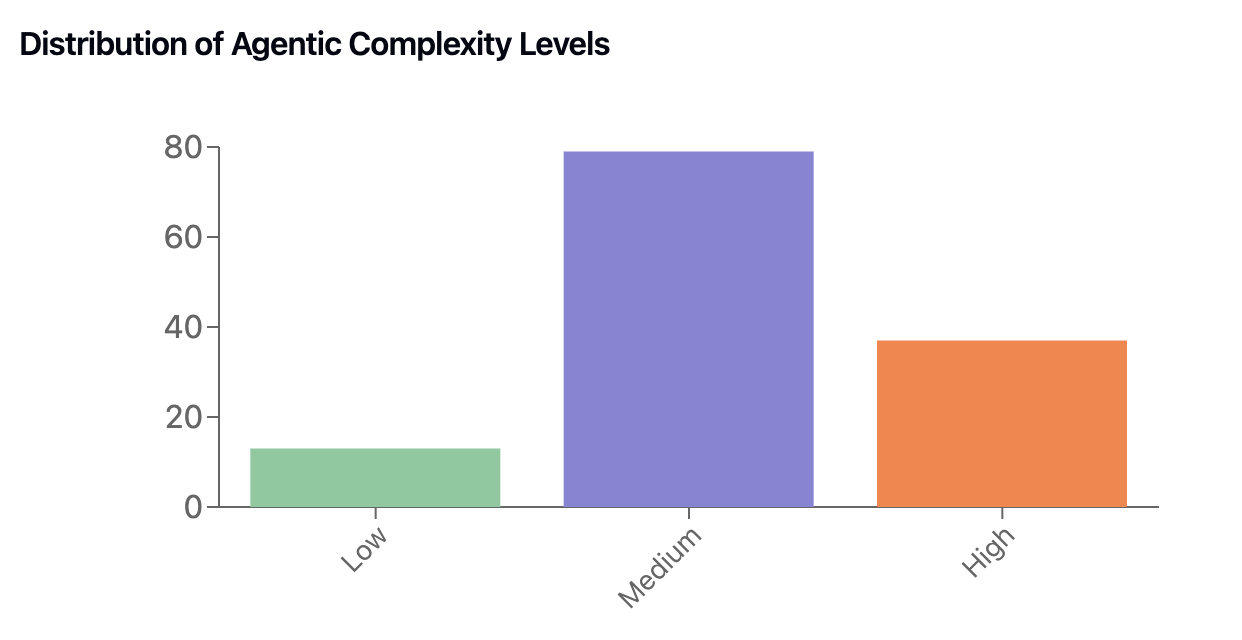
\includegraphics[width=6cm]{../agentic-complexity-levels.png}\includegraphics[width=6cm]{../query_distribution_by_domain.png} 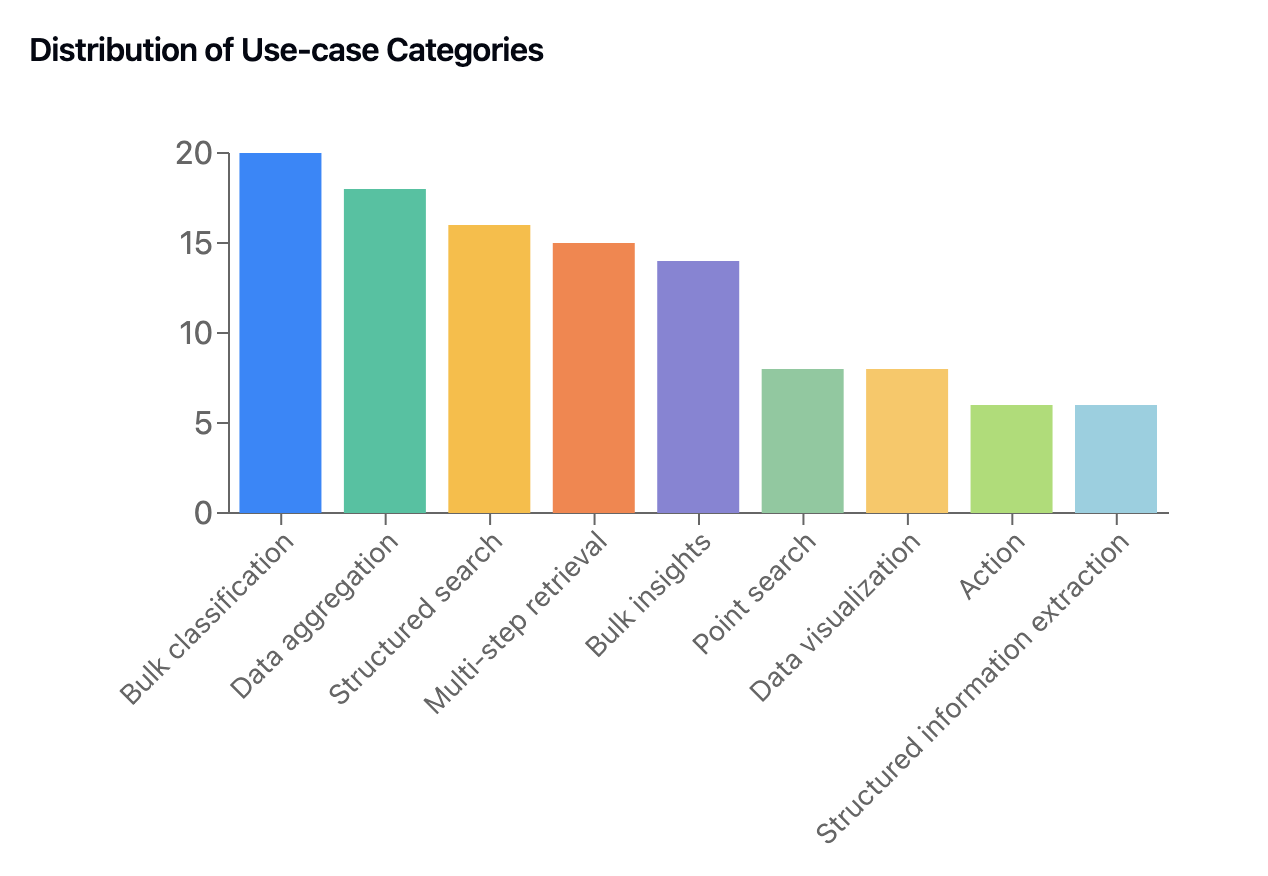
\includegraphics[width=6cm]{../use-case-category-distribution.png}
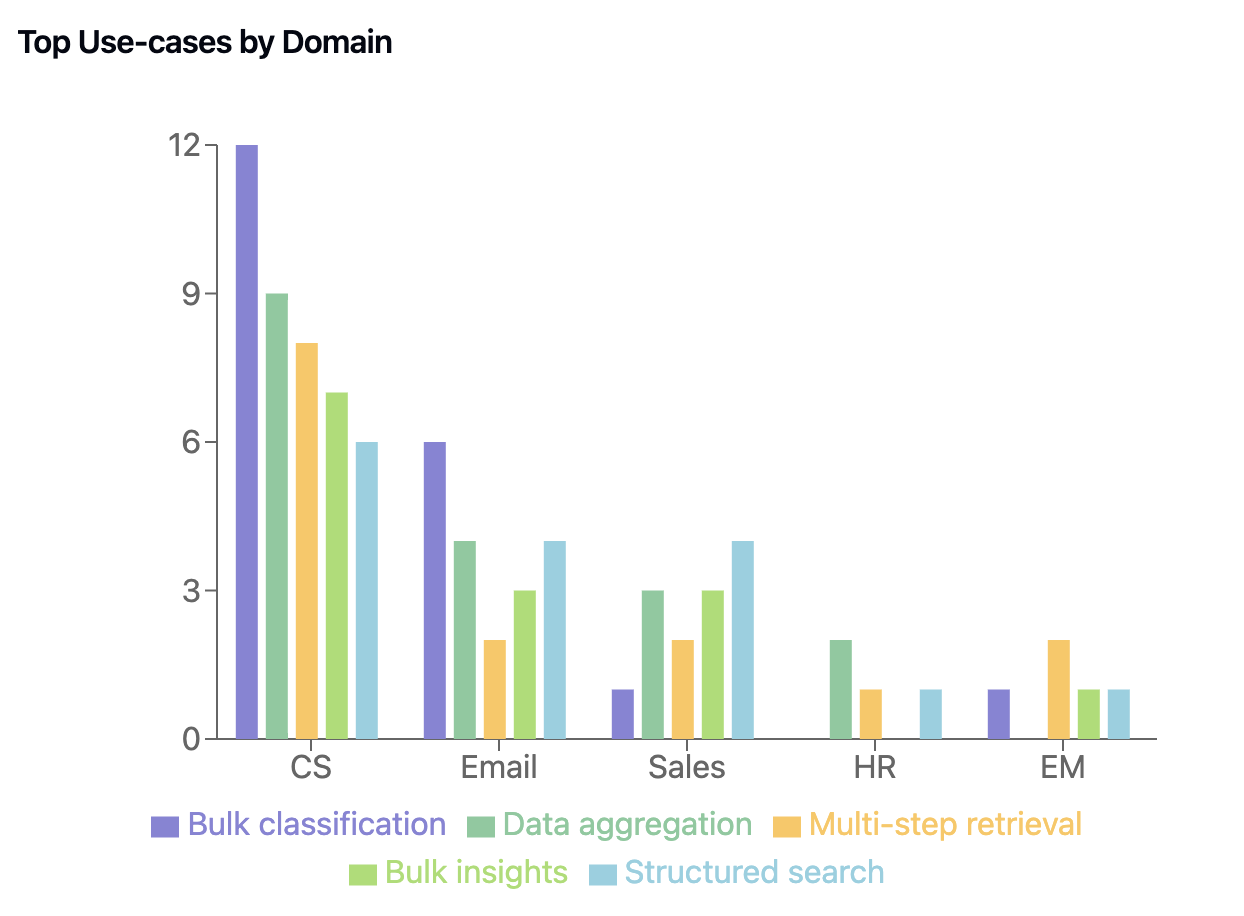
\includegraphics[width=6cm]{../use-cases-by-domain.png}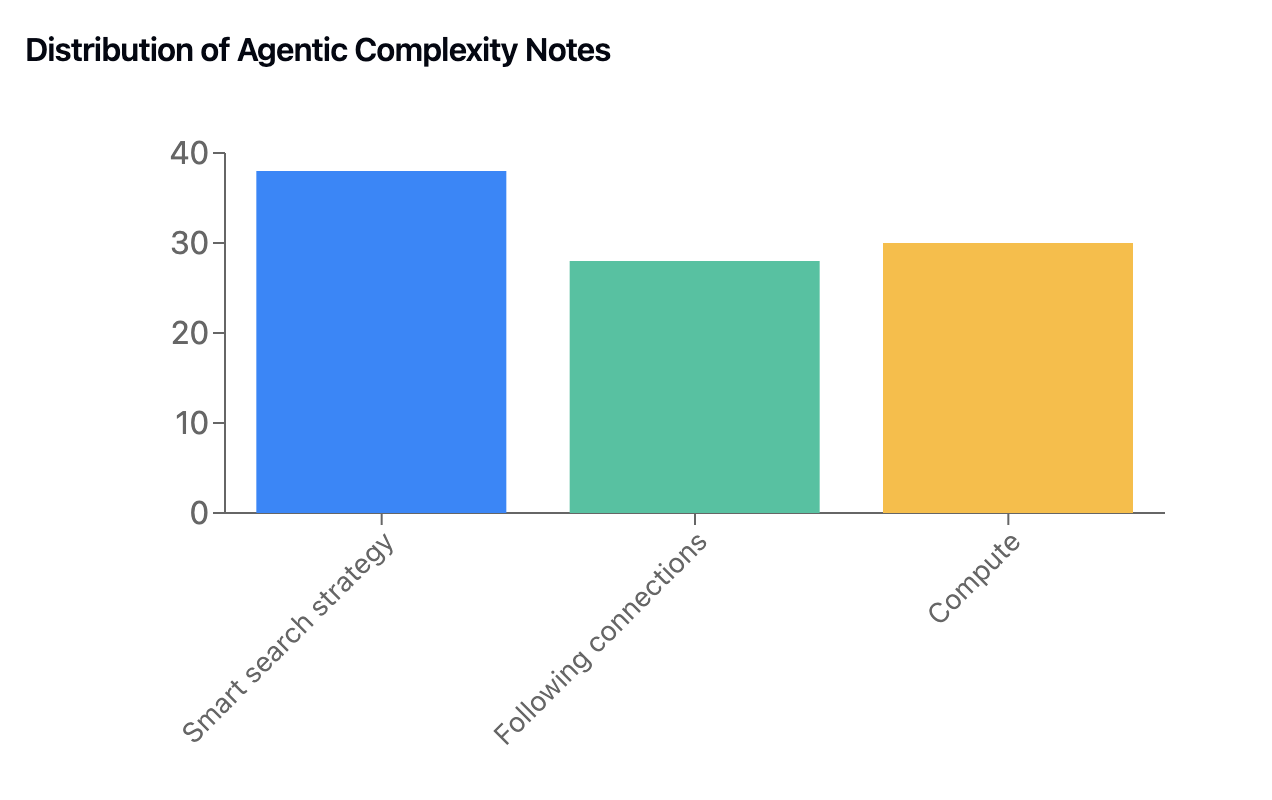
\includegraphics[width=6cm]{../agentic-complexity-types.png}\includegraphics[width=6cm]{../complexity-levels-by-domain.png}

%\begin{figure}[htbp]
%    \centering
%    \begin{subfigure}[b]{0.45\textwidth}
%        \includegraphics[width=\textwidth]{query_distribution_by_domain.png}
%        \caption{Question distribution by domain}
%    \end{subfigure}
%    \hfill
%    \begin{subfigure}[b]{0.45\textwidth}
%        \includegraphics[width=\textwidth]{complexity-levels-by-domain.png}
%        \caption{Question distribution by complexity}
%    \end{subfigure}
%\end{figure}

\section{Evaluation Methodology}

The Data Access Agent Benchmark employs a goal-oriented evaluation metric\cite{42}, recognizing that while many dataset questions could be approached in a zero-shot (or question-answer) setting, users typically interact with the agent through an assistant. This interaction often evolves into a dialogue where users provide helpful hints to guide task completion based on previous responses.\\

Most evaluation studies on dialogue systems follow the PARADISE\cite{43} framework. This framework evaluates user satisfaction through two key metrics: dialogue cost and task success. Dialogue cost measures interaction costs, such as the number of conversation turns, while task success assesses whether the system successfully achieves the user's goal. We can use a weighted combination of both metrics to come up with an overall score, although we believe that the task success alone may be reasonably considered as the main metric.\\

Given the challenges of evaluating dialogue responses on enterprise settings\cite{19}, we will mainly rely on human assessment of the dialogues to measure the metrics.

\section{Discussion: Technical Approaches and their Limitations}

We will briefly overview few common approaches to build systems on enterprise data and discuss their limitations.

\textit{RAG}: RAG is a type of retrieval-augmented approach\cite{10},\cite{11},\cite{36} where text-embedding based search is used to enhance the grounding of the responses generated by the LLM. More recently, techniques like GraphRAG\cite{41} aim to augment text-embedding search with other techniques (like building knowledge graphs) to improve task performance. Although few use-cases like information search (described later) cater well to RAG approaches, it faces key limitations: lack of temporal awareness and attribute filtering, challenging to maintain user authorization with embeddings based search, and perhaps most importantly: limited to textual data.

\textit{text-to-SQL}: Database question-answering leverages text-to-SQL\cite{12} systems for data retrieval, but is limited in it's scope. The reality of  enterprise data is that it's usually spread across multiple databases and is stored in different column formats (complex types like JSON/STRUCT also becoming quite common). Moreover, SQL systems can only ever answer filter-based search or data aggregation kind of questions. SQL's inherent limitations make it unsuitable for tasks like summarization, classification and business-logic based computations.

\textit{Tool use}: Tool use\cite{25}, \cite{30} in LLMs provides the most flexible approach for retrieving data and executing tasks, but faces practical challenges: missing APIs, poor documentation for APIs, and increased hallucination risk when handling large data inputs for these tools. These limitations significantly impact the reliability of tool use based approaches in real-world environments.


\section{Extending DAAB and Future Work}



\section{Conclusion}

The Data Access Agent Benchmark represents a significant step forward in evaluating enterprise AI systems' ability to work with private data. By providing a standardized way to assess these capabilities, we hope to drive progress in building more effective enterprise AI solutions that can truly understand and work with organizational data.

The complete benchmark dataset is available at [TODO: Add link to dataset].

We invite the AI community to use this benchmark in evaluating their enterprise AI systems and welcome feedback on making it even more useful for measuring progress in this crucial area.



\printbibliography

\end{document}

